% \begin{frame}{Formal Setting}
%   \begin{itemize}
%     \item measure space, probability measure, random vector, subvector, complementary vector, pdf
%     \item measure space of square integrable functions
%     \item inner product
%     \item norm
%   \end{itemize}
  
% \end{frame}

\begin{frame}{Decomposition of Model into Interpretable Components} % What is it?
\begin{block}{General Form}
\[
  \begin{aligned}
    y(\boldsymbol{X}) 
    &= \sum_{u \subseteq \{1,\dots,N\}} y_{u}(\boldsymbol{X}_u) \\[3pt]
    &\uncover<3->{= y_{\emptyset} 
       + \big( y_{\{1\}}(X_1) + \dots + y_{\{N\}}(X_N) \big)} \\[2pt]
    &\uncover<4->{\quad + \big( y_{\{1, 2\}}(X_1,X_2) 
                 + y_{\{1, 3\}}(X_1,X_3) + \dots \big)} \\[2pt]
    &\uncover<5->{\quad + \big( y_{\{1, 2, 3\}}(X_1,X_2,X_3) + \dots \big) 
       + \dots + y_{\{1, \dots, N\}}(X_1, \dots, X_N)}
  \end{aligned}
\]
\end{block}

\begin{itemize}
  \item<2-> $y : \text{Model}$
  \item<2-> $y_u : \text{Component functions for subvector } \boldsymbol{X}_u$
  \item<2-> $\boldsymbol{X} = (X_1, \dots, X_N)$: input variables (assumed to be independent in classical fANOVA)
\end{itemize}
\end{frame}

\begin{frame}{Conditions for Interpretability under Independent Inputs} % What conditions do we need?
  \begin{block}{Strong Annihilating Conditions}
    \[
      \int_{\mathbb{R}} y_u(\boldsymbol{x}_u) f_{\{i\}}(x_i) \, d\nu(x_i) = 0 
      \quad \text{for} \ i \in u \neq \emptyset
    \]
  \end{block}

  \begin{itemize}
    \item<2-> $f_{\{i\}}$ : marginal density of variable $X_i$
    \item<2-> $\nu$: reference measure on $\mathbb{R}$; $d\nu(x_i)$ indicates integration with respect to $\nu$ in the variable $x_i$
  \end{itemize}

  \uncover<3->{It follows:}
  \begin{align*}
    \uncover<3->{\mathbb{E}[y_u(\boldsymbol{X}_u)] = 0}
  \end{align*}
  \begin{align*}
    \uncover<4->{\mathbb{E}[y_u(\boldsymbol{X}_u) y_v(\boldsymbol{X}_v)] = 0 \quad (u \neq v)}
  \end{align*}
\end{frame}


\begin{frame}{Recursive Form of the Components}
    % y_emptyset always visible
    \[
    y_{\emptyset} = \int_{\mathbb{R}^N} y(\boldsymbol{x}) 
    \prod_{i=1}^{N} f_{\{i\}}(x_i) \, d\nu (x_i) 
    = \mathbb{E}[y(\boldsymbol{X})]
    \]

    % Single align with overlays
    \begin{align*}
        \onslide<3->{%
        y_u(\boldsymbol{X}_u) 
        &= \int_{\mathbb{R}^{N- |u|}} 
            y(\boldsymbol{X}_u, \boldsymbol{x}_{-u}) 
            \prod_{i=1, i \notin u}^{N} f_{\{i\}}(x_i) 
            \, d\nu (x_i) 
          - \sum_{v \subsetneq u} y_v(\boldsymbol{X}_v) 
        } \\[0.5em]
        \onslide<4->{%
        &= \mathbb{E}[y(\boldsymbol{X}_{u}, \boldsymbol{X}_{-u}) 
           \mid \boldsymbol{X}_u = \boldsymbol{x}_u]
           - \sum_{v \subsetneq u} y_v(\boldsymbol{X}_v)
        }
    \end{align*}

    \uncover<2->{
        \begin{itemize}
        \item \(f_{\boldsymbol{X}}(\boldsymbol{x})\,d\nu(\boldsymbol{x})
               = \prod_{i=1}^{N} f_{\{i\}}(x_i)\,d\nu(x_i)\)
        \item \(f_{\boldsymbol{X}}(\boldsymbol{x})\,d\nu (\boldsymbol{x}_{-u})
               = \prod_{i=1, i \notin u}^{N} f_{\{i\}}(x_i)\,d\nu(x_i)\)
    \end{itemize}
    }

\end{frame}



\begin{frame}{Example of Recursive Form}
  \begin{itemize}
    \item<1-> $N = 3$, $u = \emptyset$
  \end{itemize}
  \uncover<2->{
    \[
    y_{\emptyset} 
      = \int_{\mathbb{R}^3} y(\boldsymbol{x}) 
        \prod_{i=1}^{3} f_{\{i\}}(x_i) \, d\nu (x_i) 
      = \mathbb{E}[y(\boldsymbol{X})]
    \]
  }

  \begin{itemize}
    \item<3-> $u = \{1\}$ $\rightarrow$ $v \in \{\emptyset\}$
  \end{itemize}
  \uncover<4->{
    \[
    y_{\{1\}}(x_1) 
      = \int_{\mathbb{R}^{2}} 
          y(x_{1}, x_{2}, x_{3}) 
          \prod_{i=2}^{3} f_{\{i\}}(x_i) \, d\nu (x_i) 
        -  y_{\emptyset}
      = \mathbb{E}[y(X_1, X_2, X_3)|X_1 = x_1] - y_{\emptyset}
    \]
  }

    \begin{itemize}
    \item<5-> $u = \{2\}$ $\rightarrow$ $v \in \{\emptyset\}$
  \end{itemize}
  \uncover<6->{
    \[
    y_{\{2\}}(x_2) 
      = \int_{\mathbb{R}^{2}} 
          y(x_{1}, x_{2}, x_{3}) 
          \prod_{i=1, i \neq 2}^{3} f_{\{i\}}(x_i) \, d\nu (x_i) 
        -  y_{\emptyset}
      = \mathbb{E}[y(X_1, X_2, X_3)|X_2 = x_2] - y_{\emptyset}
    \]
  }
\end{frame}

\begin{frame}
    \begin{itemize}
    \item $u = \{1,2\}$ $\rightarrow$ $v \in \{\emptyset, \{1\}, \{2\}\}$
  \end{itemize}
  \uncover<2->{
    \begin{align*}
    y_{\{1,2\}}(x_1, x_2) 
      &= \int_{\mathbb{R}} 
          y(x_1, x_2, x_3) 
          f_{\{3\}}(x_3) \, d\nu (x_3) 
        -  y_{\{1\}}(x_1) -  y_{\{2\}}(x_2) - y_{\emptyset} \\[3pt]
      &= \mathbb{E}[y(X_1, X_2, X_3)|X_1 = x_1, X_2 = x_2] 
        - y_{\{1\}}(x_1) - y_{\{2\}}(x_2) - y_{\emptyset}
    \end{align*}
  }
  \begin{itemize}
      \item<3-> $u = \{1, 2, 3\}$ $\rightarrow$ $v \in \{\emptyset, \{1\}, \{2\}, \{3\}, \{1, 2\}, \{1, 3\}, \{2, 3\}\}$
  \end{itemize}
  \uncover<4->{
    \begin{align*}
    y_{\{1,2,3\}}(x_1, x_2, x_3) 
      &= y(x_1, x_2, x_3)
        -  y_{\{1\}}(x_1) -  y_{\{2\}}(x_2) - y_{\{3\}}(x_3) - y_{\emptyset} \\[3pt]
      &- y_{\{1, 2\}}(x_1, x_2) - y_{\{1, 3\}}(x_1, x_3) - y_{\{2, 3\}}(x_2, x_3) 
    \end{align*}
  }
  \uncover<5->{Remark: fANOVA components can be seen from the lens of orthogonal projections.}
\end{frame}


\begin{frame}{Example with Independent MVN Input} % Example of a 2D function
  \uncover<1->{
    \begin{align*}
      y(x_1, x_2) = 2x_1 + x_2^{2} + x_1 x_2
    \end{align*}
  }

  \uncover<2->{
    \[
    (X_1, X_2)^\mathsf{T} \sim 
    \mathcal{N}\!\left(
      \begin{pmatrix}0 \\ 0\end{pmatrix},
      \begin{pmatrix}
        1 & 0 \\ 
        0 & 1
      \end{pmatrix}
    \right)
    \]
  }

  \uncover<3->{
    \[
    X_1 \mid X_2=x_2 \sim \mathcal{N}(0, 1), 
    \quad
    X_2 \mid X_1=x_1 \sim \mathcal{N}(0, 1)
    \]
  }

  \uncover<4->{Components:}
  \uncover<5->{
    \begin{equation*}
      y_{\emptyset} = 1, \qquad
      y_{\{1\}}(x_1) = 2x_1, \qquad
      y_{\{2\}}(x_2) = x_2^{2} - 1, \qquad
      y_{\{1,2\}}(x_1, x_2) = x_1 x_2
    \end{equation*}
  }
\end{frame}


\begin{frame}{Visualization of fANOVA components under Independence}
  \begin{align*}
    y(x_1, x_2) = 2x_1 + x_2^{2} + x_1 x_2
  \end{align*}
  \begin{columns}
    \column{0.5\textwidth}
      \centering
      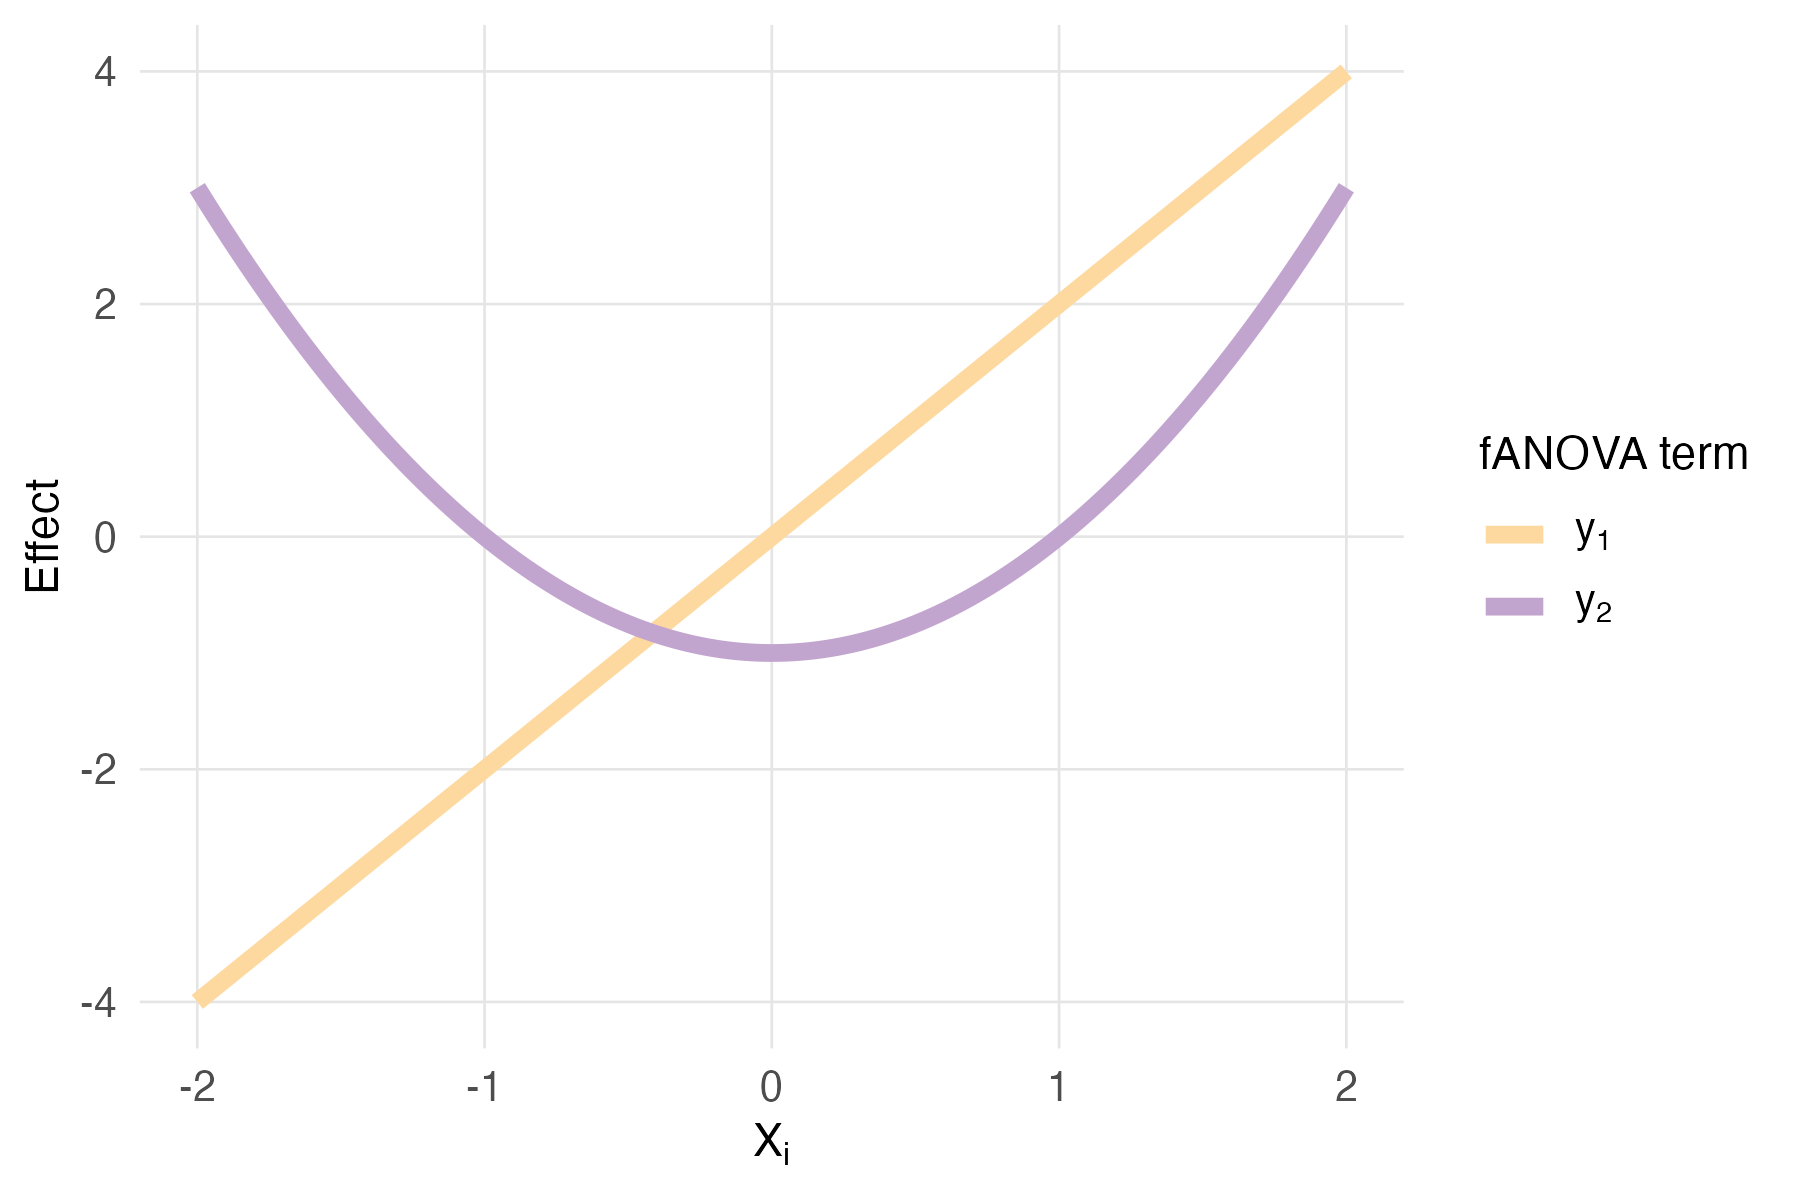
\includegraphics[width=\linewidth]{../images/experiment_section/classical_ex_1_a1p20_a2p00_a11p00_a22p10_a12p10_rhop00_main.png}
    \column{0.5\textwidth}
      \centering
      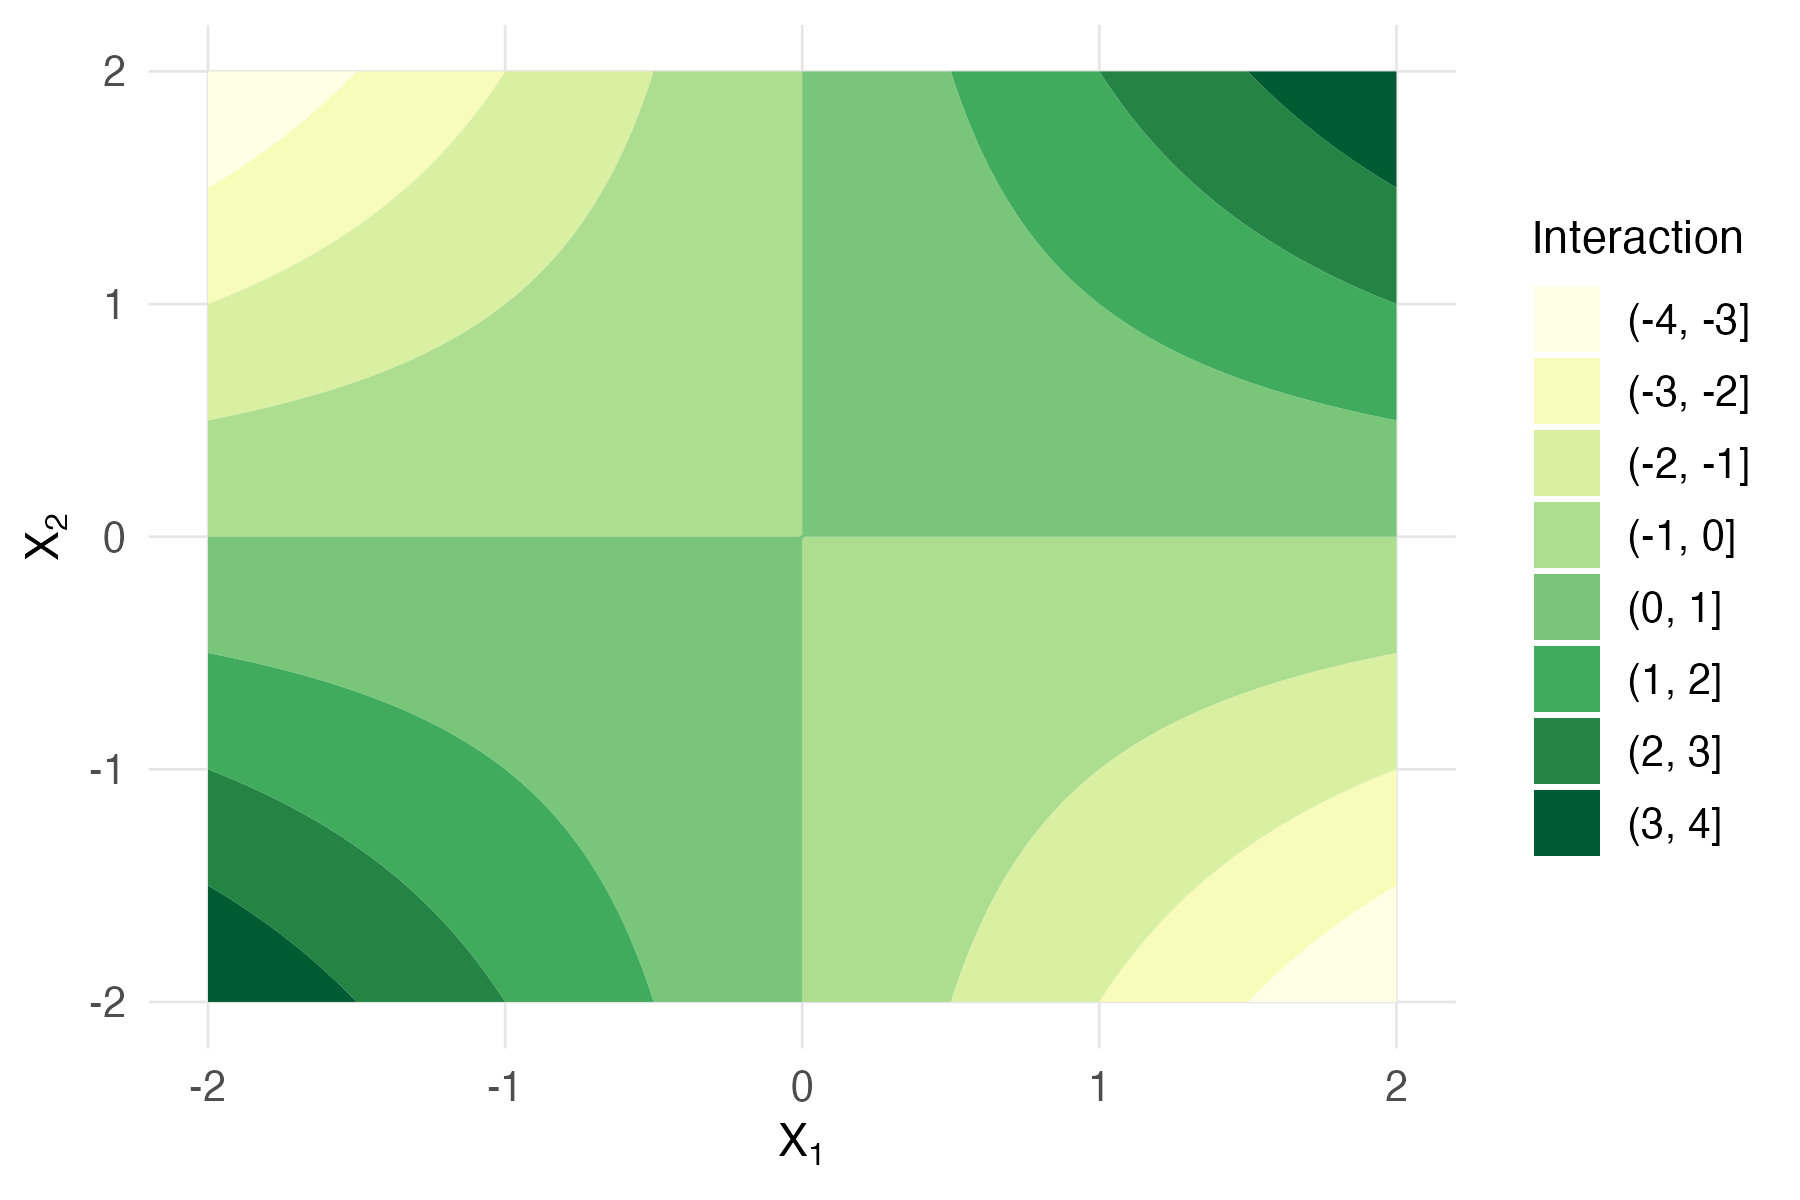
\includegraphics[width=\linewidth]{../images/experiment_section/classical_ex_1_a1p20_a2p00_a11p00_a22p10_a12p10_rhop00_interaction.png}
  \end{columns}
\end{frame}





% fANOVA through lens of Orthogonal Projections
